\documentclass[12pt,a4paper]{article}

% ─── Pacotes principais ───────────────────────────────────────────────────────
\usepackage[utf8]{inputenc}
\usepackage[T1]{fontenc}
\usepackage[brazil]{babel}
\usepackage{lmodern}
\usepackage{geometry}
\geometry{a4paper, top=2.5cm, bottom=2.5cm, left=3cm, right=2.5cm}

% ─── Tipografia e layout ──────────────────────────────────────────────────────
\usepackage{setspace}
\onehalfspacing
\usepackage{indentfirst}
\usepackage{microtype}

% ─── Matemática ───────────────────────────────────────────────────────────────
\usepackage{amsmath}
\usepackage{amssymb}
\usepackage{mathtools}

% ─── Gráficos e cores ─────────────────────────────────────────────────────────
\usepackage{graphicx}
\usepackage{xcolor}
\definecolor{azul}{RGB}{0,70,127}
\definecolor{cinza}{RGB}{100,100,100}
\definecolor{verde}{RGB}{0,120,60}

% ─── Tabelas ──────────────────────────────────────────────────────────────────
\usepackage{booktabs}
\usepackage{multirow}
\usepackage{array}
\usepackage{tabularx}
\usepackage{longtable}
\newcolumntype{C}[1]{>{\centering\arraybackslash}p{#1}}
\newcolumntype{L}[1]{>{\raggedright\arraybackslash}p{#1}}
\newcolumntype{R}[1]{>{\raggedleft\arraybackslash}p{#1}}

% ─── TikZ para diagramas ──────────────────────────────────────────────────────
\usepackage{tikz}
\usetikzlibrary{shapes.geometric, arrows.meta, positioning, fit,
                decorations.pathreplacing, backgrounds, calc}

% ─── PGFPlots para gráficos ───────────────────────────────────────────────────
\usepackage{pgfplots}
\pgfplotsset{compat=1.18}
\usepackage{pgfplotstable}

% ─── Código-fonte ─────────────────────────────────────────────────────────────
\usepackage{listings}
\lstset{
  basicstyle=\ttfamily\small,
  breaklines=true,
  frame=single,
  backgroundcolor=\color{gray!8},
  keywordstyle=\color{azul}\bfseries,
  commentstyle=\color{cinza}\itshape,
  numbers=left,
  numberstyle=\tiny\color{cinza},
  xleftmargin=1.5em,
}

% ─── Hyperlinks ───────────────────────────────────────────────────────────────
\usepackage[hidelinks]{hyperref}

% ─── Cabeçalho / rodapé ───────────────────────────────────────────────────────
\usepackage{fancyhdr}
\pagestyle{fancy}
\fancyhf{}
\fancyhead[L]{\small\color{cinza}BirdSearch — Recuperação de Informação Acústica}
\fancyhead[R]{\small\color{cinza}\thepage}
\renewcommand{\headrulewidth}{0.4pt}

% ─── Caixas de destaque ───────────────────────────────────────────────────────
\usepackage{tcolorbox}
\tcbuselibrary{skins,breakable}
\newtcolorbox{destaque}[1][]{
  enhanced, breakable,
  colback=azul!5, colframe=azul!60,
  fonttitle=\bfseries\small,
  #1
}

% ─── Metadados ────────────────────────────────────────────────────────────────
\title{%
  {\Large\bfseries BirdSearch}\\[0.5em]
  {\large Sistema de Recuperação de Informação Acústica\\
  para Identificação de Espécies de Aves}\\[1.5em]
  {\normalsize Recuperação de Informação Multimídia --- BirdCLEF 2026}
}
\author{%
  Pedro Lucas Mendes\\
  \small Instituto de Computação, UFAM\\
  \small \texttt{pedro.mendes@icomp.ufam.edu.br}
}
\date{Junho de 2026}

% ══════════════════════════════════════════════════════════════════════════════
\begin{document}

\maketitle
\thispagestyle{empty}

\begin{abstract}
\noindent
Este relatório descreve o \textbf{BirdSearch}, um sistema de recuperação de
informação acústica para identificação de espécies de aves desenvolvido para
o desafio BirdCLEF 2026. O sistema implementa um \emph{framework} modular e
orientado a configuração que cobre todas as etapas do pipeline de RI:
pré-processamento, segmentação temporal, extração de embeddings neurais,
representação de documentos, indexação vetorial, fusão de evidências e
\emph{reranking}. Duas estratégias centrais de indexação são avaliadas:
\textbf{E1} (\emph{late fusion} por segmentos, índice HNSW) e \textbf{E2}
(\emph{early fusion} via super-embedding, índice plano). Os experimentos com
dois \emph{backbones} neurais --- Google Perch v2 (1280 dim) e BirdNET v3.0
(1280 dim) --- sobre um corpus de 34.144 gravações (571 espécies) revelam que:
(i) E2 lidera em MAP (0,8227 \emph{vs.}\ 0,8191 em E1) e latência (6,3~ms
\emph{vs.}\ 22,6~ms); (ii) rerankers baseados em \emph{score} (\texttt{attention}:
MAP\,=\,0,8944 com BirdNET; MAP\,=\,0,8689 com Perch v2) superam fusão por
rank em MAP/MRR; (iii) \texttt{taxonomy\_boost} maximiza métricas
biologicamente orientadas (genus@5\,$>$\,0,92, common@10\,$>$\,0,94); e (iv)
híbridos combinam qualidade comparável a rerankers simples com latência de
0,3--1,0~ms.
\end{abstract}

\tableofcontents
\newpage

% ══════════════════════════════════════════════════════════════════════════════
\section{Introdução}
\label{sec:intro}
% ══════════════════════════════════════════════════════════════════════════════

A bioacústica computacional é um campo em rápido crescimento que aplica técnicas
de processamento de sinais e aprendizado de máquina para analisar sons de
animais. A identificação automática de espécies de aves a partir de gravações
acústicas constitui, em particular, um problema de \emph{recuperação de
informação} (RI) multimídia com impacto direto em monitoramento ambiental,
conservação da biodiversidade e estudos ecológicos de larga escala. Plataformas
como a Xeno-canto já reúnem mais de 700.000 gravações de mais de 10.000 espécies,
tornando a busca eficiente nessa coleção um desafio não trivial.

O desafio \textbf{BirdCLEF 2026} fornece um \emph{benchmark} padronizado com
34.144 gravações de campo para 571 espécies da região amazônica. O objetivo é,
dada uma gravação de consulta, recuperar e ranquear as espécies mais prováveis
do corpus. Esse cenário diferencia-se de tarefas de classificação clássica pois:
(a) o espaço de classes é aberto e muda entre splits; (b) cada gravação pode
conter vocalizações de múltiplas espécies; e (c) a duração dos arquivos é
variável, exigindo estratégias de segmentação.

O \textbf{BirdSearch} aborda esse problema com um \emph{framework} de RI acústico
modular, config-driven, construído sobre dois eixos investigativos principais:

\begin{enumerate}
  \item \textbf{Estrutura do índice e fusão de evidências}: como organizar os
  embeddings de múltiplos segmentos de um mesmo áudio no índice vetorial e como
  combinar evidências parciais durante a recuperação.
  \item \textbf{Reranking}: como reposicionar candidatos após a busca vetorial
  para maximizar precisão e relevância biológica.
\end{enumerate}

O sistema avalia 19 estratégias de \emph{ranking}/\emph{reranking} sobre dois
\emph{backbones} de embedding --- Google Perch v2~\cite{merriënboer:25} e
BirdNET v3.0~\cite{kahl:21} --- medindo quatro famílias de métricas: ranking
global (MAP, MRR, nDCG), recall posicional (P@k, R@k), proximidade
taxonômica (genus@k, common@k) e latência de busca.

\paragraph{Organização.}
A Seção~\ref{sec:fundamentacao} apresenta os fundamentos teóricos e as métricas.
A Seção~\ref{sec:arquitetura} descreve a arquitetura do sistema e cada estágio
do pipeline. A Seção~\ref{sec:indexacao} detalha as estratégias de indexação.
A Seção~\ref{sec:reranking} apresenta os rerankers implementados. A
Seção~\ref{sec:experimentos} descreve a configuração experimental. A
Seção~\ref{sec:resultados} apresenta e discute os resultados. A
Seção~\ref{sec:conclusao} conclui o trabalho.

% ══════════════════════════════════════════════════════════════════════════════
\section{Fundamentação Teórica e Métricas de Avaliação}
\label{sec:fundamentacao}
% ══════════════════════════════════════════════════════════════════════════════

\subsection{Recuperação de Informação por Similaridade Vetorial}

A recuperação de informação por similaridade (ou \emph{nearest-neighbor
retrieval}) consiste em, dado um vetor de consulta $\mathbf{q} \in \mathbb{R}^d$
e uma coleção de vetores de documentos $\{\mathbf{d}_1,\ldots,\mathbf{d}_N\}
\subset \mathbb{R}^d$, encontrar os $k$ vetores mais similares a $\mathbf{q}$
segundo uma função de similaridade $\sigma$. Neste trabalho adotamos a
\textbf{similaridade cosseno}:
\begin{equation}
  \sigma_{\cos}(\mathbf{q}, \mathbf{d}) =
  \frac{\mathbf{q} \cdot \mathbf{d}}{\|\mathbf{q}\|\,\|\mathbf{d}\|}
  \label{eq:cosine}
\end{equation}

Como os embeddings do Perch v2 e do BirdNET são L2-normalizados
($\|\mathbf{q}\| = \|\mathbf{d}\| = 1$), a Equação~\eqref{eq:cosine} reduz-se
ao produto interno:
\begin{equation}
  \sigma_{\cos}(\mathbf{q}, \mathbf{d}) = \mathbf{q} \cdot \mathbf{d}
  \label{eq:inner}
\end{equation}

Isso permite que todos os índices FAISS usem \texttt{IndexFlatIP} (produto
interno), tratando a busca cosseno como busca euclidiana normalizada.

\subsection{Métricas de Avaliação}

\subsubsection{Average Precision e MAP}

Para uma consulta com rótulo verdadeiro $\ell$, seja $\mathbf{r} =
(r_1,\ldots,r_k)$ a lista de resultados recuperados. Defina a relevância
binária $\text{rel}(r_i) = \mathbf{1}[\text{label}(r_i) = \ell]$. A
\textbf{Average Precision} (AP) é:
\begin{equation}
  \text{AP} =
  \frac{1}{\min(|\mathcal{R}_\ell|, k)}
  \sum_{i=1}^{k} \text{rel}(r_i) \cdot
  \frac{\sum_{j=1}^{i} \text{rel}(r_j)}{i}
  \label{eq:ap}
\end{equation}
onde $\mathcal{R}_\ell$ é o conjunto de documentos relevantes do corpus
(todos que compartilham o rótulo $\ell$). A AP penaliza fortemente resultados
relevantes em posições tardias e recompensa listas bem ordenadas.

O \textbf{Mean Average Precision} (MAP) é a média das APs sobre todas as
consultas $Q$:
\begin{equation}
  \text{MAP} = \frac{1}{|Q|}\sum_{q \in Q} \text{AP}(q)
  \label{eq:map}
\end{equation}

\subsubsection{Mean Reciprocal Rank}

O \textbf{MRR} foca no rank da primeira resposta correta:
\begin{equation}
  \text{MRR} = \frac{1}{|Q|}\sum_{q \in Q} \frac{1}{\text{rank}_q^*}
  \label{eq:mrr}
\end{equation}
onde $\text{rank}_q^*$ é a posição (1-indexada) do primeiro documento relevante
para $q$, e $1/\text{rank}_q^* = 0$ se não houver nenhum. No cenário do
BirdSearch, em que há pelo menos um documento correto por consulta, MAP e MRR
convergem numericamente (pois a lista é dominada pelo primeiro acerto).

\subsubsection{nDCG}

O \textbf{Normalized Discounted Cumulative Gain} generaliza a AP com um desconto
logarítmico por posição:
\begin{equation}
  \text{DCG}@k = \sum_{i=1}^{k}
  \frac{2^{\text{rel}(r_i)} - 1}{\log_2(i + 1)}
  \label{eq:dcg}
\end{equation}
\begin{equation}
  \text{nDCG}@k = \frac{\text{DCG}@k}{\text{IDCG}@k}
  \label{eq:ndcg}
\end{equation}
onde IDCG@k é o DCG do ranking ideal (todos os documentos relevantes no topo).
O desconto $1/\log_2(i+1)$ penaliza resultados corretos encontrados em posições
tardias: posição 1 pesa 1,0; posição 2 pesa $\approx$0,63; posição 10 pesa
$\approx$0,29.

\subsubsection{Precision@k e Recall@k}

\begin{align}
  \text{P@}k &= \frac{|\{r_1,\ldots,r_k\} \cap \mathcal{R}_\ell|}{k}
  \label{eq:patk}\\[4pt]
  \text{R@}k &= \frac{|\{r_1,\ldots,r_k\} \cap \mathcal{R}_\ell|}
                    {\max(1,|\mathcal{R}_\ell|)}
  \label{eq:ratk}
\end{align}

Uma sutileza importante: o denominador de R@k depende da representação
de documentos. Na representação \emph{audio} (um doc por arquivo), há um
documento relevante por consulta, de modo que R@1 equivale a P@1. Já na
representação \emph{segment} (um doc por segmento), $|\mathcal{R}_\ell|$ pode
chegar a centenas, tornando o recall muito menor. As duas estratégias devem
ser comparadas com cautela nessa métrica.

\subsubsection{Métricas Taxonômicas}

Além das métricas clássicas de RI, o BirdSearch avalia \textbf{proximidade
biológica}. Definimos:
\begin{align}
  \text{genus@}k &= \frac{1}{|Q|}\sum_q
    \frac{|\{r \in \text{top-}k : \text{genus}(r) = \text{genus}(q)\}|}{k}
  \label{eq:genusk}\\[4pt]
  \text{common@}k &= \frac{1}{|Q|}\sum_q
    \frac{|\{r \in \text{top-}k : \text{tokens}(r) \cap \text{tokens}(q) \neq \emptyset\}|}{k}
  \label{eq:commonk}
\end{align}
onde $\text{tokens}(s)$ são os tokens do nome comum da espécie $s$. Essas
métricas capturam utilidade para um ornitólogo: mesmo sem identificar a espécie
exata, resultados do mesmo gênero têm valor biológico.

\subsubsection{Latência}

Medida via \texttt{perf\_counter} em milissegundos somente sobre a chamada ao
\texttt{Retriever.retrieve} (busca + ranking; \emph{não} inclui tempo de
embedding). Reportamos: média, p50, p95 e p99.

% ══════════════════════════════════════════════════════════════════════════════
\section{Arquitetura do Sistema}
\label{sec:arquitetura}
% ══════════════════════════════════════════════════════════════════════════════

\subsection{Visão Geral}

O BirdSearch é organizado em um pipeline sequencial de oito estágios
independentes, conectados por um \textbf{padrão de registro} central. A
Figura~\ref{fig:pipeline} mostra o diagrama arquitetural completo.

% ─── Diagrama do pipeline ─────────────────────────────────────────────────────
\begin{figure}[htbp]
\centering
\begin{tikzpicture}[
    node distance=0.55cm and 0.7cm,
    stage/.style={
      rectangle, rounded corners=4pt,
      draw=azul!70, fill=azul!8,
      minimum width=2.6cm, minimum height=0.9cm,
      font=\small\bfseries, text centered,
      inner sep=4pt
    },
    arrow/.style={-Stealth, thick, color=azul!70},
    label/.style={font=\scriptsize\itshape, color=cinza},
    group/.style={draw=gray!40, dashed, rounded corners, inner sep=6pt}
  ]

  % Train path
  \node[stage] (load)    {Carregamento\\de Dados};
  \node[stage, below=of load] (split) {Divisão\\Treino/Teste};

  % Train branch
  \node[stage, below left=0.8cm and 1.4cm of split] (preproc_tr) {Pré-proc.\\(Treino)};
  \node[stage, below=of preproc_tr] (seg_tr)    {Segmentação\\(Treino)};
  \node[stage, below=of seg_tr]     (emb_tr)    {Embedding\\Perch v2 / BirdNET};
  \node[stage, below=of emb_tr]     (docstore)  {Doc Store\\(Representação)};
  \node[stage, below=of docstore]   (index)     {Índice Vetorial\\(HNSW / Flat)};

  % Test / Query branch
  \node[stage, below right=0.8cm and 1.4cm of split] (preproc_te) {Pré-proc.\\(Teste)};
  \node[stage, below=of preproc_te] (seg_te)    {Segmentação\\(Teste)};
  \node[stage, below=of seg_te]     (emb_te)    {Embedding\\(Consulta)};
  \node[stage, below=of emb_te]     (fusion)    {Fusão\\(Early / Late)};

  % Shared retrieval
  \node[stage, below right=0.9cm and 0.0cm of index] (retriever) {Recuperação\\(kNN)};
  \node[stage, below=of retriever]  (ranker)    {Reranking};
  \node[stage, below=of ranker]     (eval)      {Avaliação\\(MAP, MRR, nDCG\ldots)};

  % Arrows – left branch
  \draw[arrow] (load)       -- (split);
  \draw[arrow] (split)      -| (preproc_tr);
  \draw[arrow] (preproc_tr) -- (seg_tr);
  \draw[arrow] (seg_tr)     -- (emb_tr);
  \draw[arrow] (emb_tr)     -- (docstore);
  \draw[arrow] (docstore)   -- (index);

  % Arrows – right branch
  \draw[arrow] (split)      -| (preproc_te);
  \draw[arrow] (preproc_te) -- (seg_te);
  \draw[arrow] (seg_te)     -- (emb_te);
  \draw[arrow] (emb_te)     -- (fusion);

  % Arrows – retrieval
  \draw[arrow] (index)   |- (retriever);
  \draw[arrow] (fusion)  |- (retriever);
  \draw[arrow] (retriever) -- (ranker);
  \draw[arrow] (ranker)    -- (eval);

  % Background groups
  \begin{scope}[on background layer]
    \node[group, fit=(preproc_tr)(seg_tr)(emb_tr)(docstore)(index),
          label={[above, font=\scriptsize\bfseries, color=azul]Indexação (Treino)}] {};
    \node[group, fit=(preproc_te)(seg_te)(emb_te)(fusion),
          label={[above, font=\scriptsize\bfseries, color=verde]Consulta (Teste)}] {};
  \end{scope}

\end{tikzpicture}
\caption{Diagrama arquitetural completo do pipeline BirdSearch. Os estágios
da esquerda constroem o índice a partir do conjunto de treino; os da direita
processam as consultas do conjunto de teste. A fase de recuperação combina as
duas ramificações.}
\label{fig:pipeline}
\end{figure}

\subsection{Padrão de Registro (\emph{Registry Pattern})}

A modularidade do sistema é garantida pelo padrão de registro implementado em
\texttt{src/utils/registry.py}. Cada estágio mantém uma instância de
\texttt{Registry} que mapeia chaves de \emph{string} a classes Python:

\begin{center}
\begin{tabular}{lll}
\toprule
\textbf{Módulo} & \textbf{Registro} & \textbf{Exemplos} \\
\midrule
\texttt{src/preprocessing/} & \texttt{PREPROCESSORS}  & \texttt{none, spectral\_gating, bandpass} \\
\texttt{src/segmentation/}  & \texttt{SEGMENTERS}     & \texttt{fixed, overlapping, energy, event} \\
\texttt{src/embeddings/}    & \texttt{EMBEDDERS}      & \texttt{perch\_v2, perch\_v2\_torch, birdnet\_v3} \\
\texttt{src/aggregation/}   & \texttt{AGGREGATORS}    & \texttt{mean, max, topk, median, attention, spe} \\
\texttt{src/representation/}& \texttt{REPRESENTATIONS}& \texttt{segment, audio, species, cluster, prototype} \\
\texttt{src/indexing/}      & \texttt{INDEXES}        & \texttt{flat, ivf, hnsw} \\
\texttt{src/fusion/}        & \texttt{FUSIONS}        & \texttt{early, late} \\
\texttt{src/ranking/}       & \texttt{RANKERS}        & \texttt{rrf, attention, softmax, taxonomy\_boost} \\
\bottomrule
\end{tabular}
\end{center}

O componente \texttt{PipelineBuilder} lê um arquivo YAML de configuração e
instancia os objetos correspondentes sem nenhum \texttt{if/elif} explícito.
Trocar de estratégia requer apenas alterar o valor de uma chave no YAML.

\subsection{Pré-processamento de Áudio}

O pré-processamento opera sobre o sinal de áudio bruto antes da segmentação.
O sistema suporta três módulos:

\paragraph{Identidade (\texttt{none}).} Passa o sinal sem modificação. Usado
como linha de base para avaliar o impacto isolado do pré-processamento.

\paragraph{Filtragem por Gating Espectral (\texttt{spectral\_gating}).}
Baseado no algoritmo de redução de ruído espectral~\cite{logothetis:96}, o
módulo estima o piso de ruído a partir dos 10\% de frames STFT mais silenciosos
e atenua componentes espectrais abaixo de um limiar adaptativo:
\begin{equation}
  \hat{M}(f,t) = \max\!\left(M(f,t) - \alpha \cdot N(f),\ 0\right)
  \label{eq:specgate}
\end{equation}
onde $M(f,t)$ é a magnitude espectral, $N(f)$ é o piso de ruído estimado e
$\alpha$ é o parâmetro \texttt{prop\_decrease} (padrão 1,0). O sinal limpo é
reconstruído por ISTFT com sobreposição de janelas (\emph{overlap-add}).

\paragraph{Filtro Passa-Banda (\texttt{bandpass}).}
Filtro Butterworth de 4ª ordem entre 250~Hz e 12.000~Hz:
\begin{equation}
  H(z) = \frac{B(z)}{A(z)},\quad B,A \in \mathbb{R}^{2 \times 4}
  \label{eq:bandpass}
\end{equation}
implementado via \texttt{scipy.signal.sosfiltfilt} (filtragem de fase zero).
A faixa foi escolhida para cobrir a maioria das vocalizações de aves (200--10.000~Hz)
com margem de segurança nas bordas.

\subsection{Segmentação Temporal}

O Perch v2 opera nativamente sobre janelas de 5~s a 32~kHz (160.000 amostras).
A etapa de segmentação divide o áudio em janelas compatíveis com esse formato.

\paragraph{Segmentação Fixa (\texttt{fixed}).}
Janelas não sobrepostas de $W$ segundos. A última janela pode ser preenchida
com zeros (\texttt{pad\_last=True}) ou descartada.

\paragraph{Segmentação com Sobreposição (\texttt{overlapping}).}
Janelas deslizantes com passo $H < W$. Neste trabalho usa-se $W = 5$~s,
$H = 2{,}5$~s (sobreposição de 50\%). O número de segmentos para um áudio de
duração $D$ é:
\begin{equation}
  N_{\text{seg}} = \left\lfloor \frac{D - W}{H} \right\rfloor + 1
  \label{eq:nseg}
\end{equation}

A sobreposição garante que vocalizações que cruzam fronteiras de janela sejam
capturadas por pelo menos um segmento com representação completa.

\paragraph{Segmentação por Energia (\texttt{energy}).}
Calcula o RMS por frame de 0,5~s e seleciona janelas centradas nos frames com
energia acima do percentil 60, até \texttt{max\_segments} janelas não sobrepostas.
Útil para gravações esparsas com longos silêncios.

\paragraph{Segmentação por Eventos (\texttt{event}).}
Detecta onsets acústicos via fluxo espectral (librosa) e posiciona janelas ao
redor dos onsets detectados, com distância mínima de 1,0~s entre janelas.

\subsection{Extração de Embeddings}

\subsubsection{Google Perch v2}

O \textbf{Google Perch v2}~\cite{merriënboer:25} é um modelo de classificação
de aves treinado sobre $>400.000$ gravações da plataforma Xeno-canto. A
arquitetura é baseada em um \emph{EfficientNet} com atenção, treinado com
contrastive learning. O modelo recebe uma janela de 5~s a 32~kHz e produz
um vetor de 1280 dimensões. Segmentos mais curtos são preenchidos com zeros;
os mais longos são recortados ao centro:

\begin{equation}
  \mathbf{e} = \frac{f_{\text{Perch}}(x)}{\|f_{\text{Perch}}(x)\|_2}
  \in \mathbb{R}^{1280},\quad \|\mathbf{e}\|_2 = 1
  \label{eq:perch}
\end{equation}

O sistema carrega o modelo via \texttt{kagglehub} (caminho preferencial) ou
TF-Hub. Uma variante \texttt{perch\_v2\_torch} exporta o SavedModel para ONNX
e executa via PyTorch, com \emph{fallback} automático ao TF se o grafo contiver
operações não suportadas.

\subsubsection{BirdNET v3.0}

O \textbf{BirdNET v3.0}~\cite{kahl:21}, desenvolvido pelo Cornell Lab of
Ornithology, opera sobre janelas nativas de 3~s a 32~kHz e produz embeddings de
1280 dimensões. Por compatibilidade com o pipeline, o sistema reamostra e
adapta as janelas conforme necessário.

\subsection{Estratégias de Agregação}

Quando múltiplos segmentos precisam ser fundidos em um único vetor (nas
representações \emph{audio}, \emph{species}, \emph{cluster}, \emph{prototype}
e na fusão precoce), o sistema aplica um \textbf{agregador}:

\begin{align}
  \mathbf{v}_{\text{mean}}   &= \ell_2\!\left(\frac{1}{N}\sum_{i=1}^N \mathbf{e}_i\right)
  \label{eq:agg_mean}\\[4pt]
  \mathbf{v}_{\text{max}}    &= \ell_2\!\left(\max_{i=1}^N \mathbf{e}_i\right)
  \label{eq:agg_max}\\[4pt]
  \mathbf{v}_{\text{median}} &= \ell_2\!\left(\text{med}_{i=1}^N \mathbf{e}_i\right)
  \label{eq:agg_median}\\[4pt]
  \mathbf{v}_{\text{topk}}   &= \ell_2\!\left(\frac{1}{k}\sum_{i \in \text{top-}k} \mathbf{e}_i\right),
    \quad k=5
  \label{eq:agg_topk}
\end{align}

onde $\ell_2(\mathbf{v}) = \mathbf{v}/\|\mathbf{v}\|_2$ e o \emph{top-k} seleciona
os $k$ segmentos com maior norma L2 (proxy de energia de sinal).

O agregador \textbf{Attention} realiza uma auto-atenção leve em relação ao centróide:
\begin{align}
  \mathbf{c} &= \ell_2\!\left(\tfrac{1}{N}\textstyle\sum_i \mathbf{e}_i\right)
  \label{eq:att_centroid}\\
  \alpha_i   &= \frac{\exp\!\left(\mathbf{e}_i \cdot \mathbf{c} / \tau\right)}
                     {\sum_j \exp\!\left(\mathbf{e}_j \cdot \mathbf{c} / \tau\right)}
  \label{eq:att_score}\\
  \mathbf{v}_{\text{att}} &= \ell_2\!\left(\sum_i \alpha_i\,\mathbf{e}_i\right),
  \quad \tau = 0{,}1
  \label{eq:att_out}
\end{align}

O parâmetro de temperatura $\tau$ controla a concentração: $\tau \to 0$
seleciona o segmento mais alinhado com o centróide; $\tau \to \infty$ degrada
para média.

O agregador \textbf{SPE} (\emph{Spatial Pyramid Encoding}) realiza pooling
multi-escala temporal:
\begin{equation}
  \mathbf{v}_{\text{SPE}} = \ell_2\!\left[\,
    \text{pool}_{L_1}(\mathbf{E})\,\|\,
    \text{pool}_{L_2}(\mathbf{E})\,\|\,
    \text{pool}_{L_3}(\mathbf{E})\,\right],
  \quad L \in \{1, 2, 4\}
  \label{eq:spe}
\end{equation}
onde $\|$ denota concatenação e $\text{pool}_L$ divide a sequência de $N$
segmentos em $L$ partes iguais e aplica mean-pooling em cada parte. O vetor
de saída tem dimensão $(L_1 + L_2 + L_3) \times d = 7 \times 1280 = 8960$.

\subsection{Representações de Documentos}
\label{sub:repr}

A representação define a granularidade do índice. O sistema implementa cinco
tipos (Tabela~\ref{tab:repr}), cada um com semântica de recuperação distinta.

\begin{table}[htbp]
\centering
\caption{Representações de documentos disponíveis no BirdSearch.}
\label{tab:repr}
\begin{tabular}{L{2.2cm}L{2.5cm}L{2.5cm}L{3.5cm}}
\toprule
\textbf{Tipo} & \textbf{Docs por arquivo} & \textbf{Tamanho do índice} & \textbf{Semantics} \\
\midrule
\texttt{segment}   & $N_{\text{seg}}$ & $O(\sum N_{\text{seg}})$ & Máxima granularidade; fusão tardia \\
\texttt{audio}     & 1              & $O(n_{\text{files}})$     & Um vetor por arquivo; fusão precoce \\
\texttt{species}   & 1 por espécie  & $O(n_{\text{labels}})$    & Vetor único por espécie \\
\texttt{cluster}   & $k$ por espécie& $O(k \cdot n_{\text{labels}})$ & Centroides k-means por espécie \\
\texttt{prototype} & 1 por espécie  & $O(n_{\text{labels}})$    & Segmento mais central por espécie \\
\bottomrule
\end{tabular}
\end{table}

A representação \texttt{segment} indexa cada janela de 5~s como documento
independente (E1), produzindo 363.917 documentos no dataset completo. A
representação \texttt{audio} indexa um único vetor agregado por arquivo (E2),
com 27.309 documentos.

\subsection{Cache de Embeddings}

Para evitar recomputação, o sistema implementa um \textbf{cache keyed}:
\begin{equation}
  \text{key} = \text{hash}(\text{path},\; \text{mtime},\; \text{embedder},\;
                            \text{preproc\_id},\; \text{segmenter\_id})
  \label{eq:cachekey}
\end{equation}

O cache armazena matrizes \texttt{.npz} por áudio. Embeddings de consultas
com ruído injetado \emph{sempre} ignoram o cache para garantir frescor.

% ══════════════════════════════════════════════════════════════════════════════
\section{Estratégias de Indexação e Fusão}
\label{sec:indexacao}
% ══════════════════════════════════════════════════════════════════════════════

\subsection{Índices Vetoriais}

\subsubsection{Índice Plano (\texttt{flat})}

O índice plano usa \texttt{FAISS IndexFlatIP}: busca exata por produto interno
sobre todos os $N$ vetores. A complexidade de busca é $O(N \cdot d)$ por
consulta. Garante os $k$ vizinhos exatos, servindo como referência de qualidade
superior. Adequado para $N \lesssim 50.000$ (E2: 27.309 documentos).

\subsubsection{Índice IVF (\texttt{ivf})}

O \texttt{FAISS IndexIVFFlat} treina um quantizador grosseiro com $n_{\text{list}}
\approx \sqrt{N}$ clusters (k-means) e, na busca, examina apenas os
$n_{\text{probe}}$ clusters mais próximos da consulta. A complexidade de busca
cai para $O(n_{\text{probe}} \cdot N/n_{\text{list}} \cdot d)$, com troca
entre latência e recall controlada por $n_{\text{probe}}$.

\subsubsection{Índice HNSW (\texttt{hnsw})}

O \textbf{Hierarchical Navigable Small World}~\cite{malkov:20} é um grafo
hierárquico de aproximação para vizinhança. A construção insere cada vetor em
múltiplas camadas com $M$ conexões por nó por camada:
\begin{itemize}
  \item \texttt{M = 32}: conexões máximas por nó
  \item \texttt{ef\_construction = 200}: largura do feixe na construção
  \item \texttt{ef\_search = 64}: largura do feixe na busca
\end{itemize}

A busca tem complexidade sub-linear $O(\log N)$ em média, com recall $> 0{,}99$
para os parâmetros acima. O HNSW é essencial em E1 com 363.917 documentos, onde
a busca plana levaria $\sim$100$\times$ mais tempo.

A Figura~\ref{fig:hnsw} ilustra a estrutura hierárquica do HNSW.

\begin{figure}[htbp]
\centering
\begin{tikzpicture}[
    node/.style={circle, draw=azul!60, fill=azul!10,
                 minimum size=0.55cm, inner sep=1pt, font=\tiny},
    link/.style={-, gray!60},
    query/.style={circle, draw=red!60, fill=red!15,
                  minimum size=0.65cm, font=\tiny\bfseries},
    scale=0.95
  ]
  % Layer 2 (top)
  \node[node] (l2a) at (1,4)   {A};
  \node[node] (l2b) at (4,4)   {B};
  \node[node] (l2c) at (7,4)   {C};
  \draw[link] (l2a)--(l2b)--(l2c);
  \node[right, font=\scriptsize\color{cinza}] at (8.5,4) {Camada 2};

  % Layer 1
  \node[node] (l1a) at (0.5,2.2) {A};
  \node[node] (l1b) at (2.0,2.2) {D};
  \node[node] (l1c) at (3.5,2.2) {B};
  \node[node] (l1d) at (5.0,2.2) {E};
  \node[node] (l1e) at (6.5,2.2) {C};
  \node[node] (l1f) at (8.0,2.2) {F};
  \draw[link] (l1a)--(l1b)--(l1c)--(l1d)--(l1e)--(l1f);
  \draw[link] (l1a)--(l1c); \draw[link] (l1d)--(l1f);
  \node[right, font=\scriptsize\color{cinza}] at (8.5,2.2) {Camada 1};

  % Layer 0 (base)
  \foreach \x/\n in {0/G,1.0/A,1.8/H,2.7/D,3.5/B,4.3/I,5.2/E,6.0/J,6.8/C,7.6/F,8.4/K} {
    \node[node] at (\x,0.4) {\n};
  }
  \node[right, font=\scriptsize\color{cinza}] at (8.5,0.4) {Camada 0};

  % Query vector
  \node[query] (q) at (4,-1.0) {q};
  \draw[-Stealth, red!60, dashed, thick] (q) -- (3.5,0.4) node[midway, right, font=\scriptsize] {busca};

  % Vertical links between layers
  \draw[link, dashed] (l2a)--(l1a); \draw[link, dashed] (l2b)--(l1c);
  \draw[link, dashed] (l2c)--(l1e);

  \node[font=\scriptsize\color{azul!80}, align=center] at (4.3, -1.8)
    {Busca desce das camadas superiores (esparsas)\\até a base (densa), guiada por vizinhança gulosa};
\end{tikzpicture}
\caption{Estrutura do grafo HNSW. A busca começa nas camadas superiores
(com poucos nós, cobrindo grandes distâncias) e desce até a camada 0 (densa),
seguindo os nós mais próximos da consulta em cada camada.}
\label{fig:hnsw}
\end{figure}

\subsection{Estratégias de Fusão de Evidências}
\label{sub:fusao}

A \textbf{fusão} define como as evidências de múltiplos segmentos de uma consulta
são combinadas para produzir o ranking final.

\subsubsection{Estratégia 1 --- Fusão Tardia (\emph{Late Fusion})}

Na E1, \emph{cada segmento da consulta é tratado como uma consulta independente}.
O sistema emite $N_q$ buscas no índice (uma por segmento) e obtém $N_q$ listas
de candidatos, que são então fundidas pelo ranker:
\begin{equation}
  \text{E1}: \quad
  \underbrace{\mathbf{q}_1, \ldots, \mathbf{q}_{N_q}}_{\text{segmentos}}
  \xrightarrow{\text{kNN}} L_1, \ldots, L_{N_q}
  \xrightarrow{\text{ranker}} \text{ranking final}
  \label{eq:e1}
\end{equation}

\textbf{Vantagens}: Preserva a diversidade de evidências ao longo do áudio; um
segmento que contém a vocalização do pássaro de forma clara pode dominar o
resultado.

\textbf{Desvantagem}: $N_q$ chamadas ao índice (tipicamente 4--12 por gravação).

\subsubsection{Estratégia 2 --- Fusão Precoce (\emph{Early Fusion})}

Na E2, os embeddings de todos os segmentos da consulta são \textbf{agregados em
um único super-embedding} antes da busca:
\begin{equation}
  \text{E2}: \quad
  \underbrace{\mathbf{q}_1, \ldots, \mathbf{q}_{N_q}}_{\text{segmentos}}
  \xrightarrow{\text{agg}} \mathbf{q}_{\text{super}}
  \xrightarrow{\text{kNN}} L
  \xrightarrow{\text{ranker}} \text{ranking final}
  \label{eq:e2}
\end{equation}

A operação de agregação padrão é \texttt{max-pooling} (Equação~\ref{eq:agg_max}),
que preserva o valor máximo por dimensão, concentrando as evidências mais fortes.

\textbf{Vantagens}: Uma única chamada ao índice; latência $\approx$\,3,5$\times$
menor que E1; índice de tamanho reduzido (27.309 \emph{vs.}\ 363.917 docs).

\textbf{Desvantagem}: Perda de granularidade fina; vocalizações fracas podem
ser suprimidas pelo max-pooling.

% ══════════════════════════════════════════════════════════════════════════════
\section{Reranking}
\label{sec:reranking}
% ══════════════════════════════════════════════════════════════════════════════

O reranking é a etapa em que a lista de candidatos recuperada pelo kNN é
\textbf{reordenada} para maximizar algum critério de qualidade. O BirdSearch
implementa cinco famílias, descritas nas próximas subseções.

\subsection{Agregação por Score}

\paragraph{Max (\texttt{max}).}
Para cada espécie $\ell$ presente nas listas de resultados, o score final é o
máximo score encontrado em qualquer segmento:
\begin{equation}
  s_{\text{max}}(\ell) = \max_{j} \sigma(\mathbf{q}_j, \mathbf{d}_\ell)
  \label{eq:rk_max}
\end{equation}

\paragraph{Mean (\texttt{mean}).}
Score médio sobre todos os segmentos e documentos recuperados para $\ell$:
\begin{equation}
  s_{\text{mean}}(\ell) = \frac{1}{|\mathcal{H}_\ell|}\sum_{h \in \mathcal{H}_\ell} h.\text{score}
  \label{eq:rk_mean}
\end{equation}

\paragraph{Top-k Mean (\texttt{topk\_mean}).}
Média dos $k$ maiores scores por espécie (padrão $k=3$):
\begin{equation}
  s_{\text{topk}}(\ell) = \frac{1}{k}\sum_{i=1}^{k} \text{sorted}(\mathcal{H}_\ell)[i]
  \label{eq:rk_topk}
\end{equation}

\paragraph{Weighted Top-k (\texttt{weighted\_topk}).}
Pesos decrescentes lineares para os $k$ melhores scores:
\begin{equation}
  s_{\text{wtopk}}(\ell) =
  \frac{\sum_{i=1}^{k} w_i \cdot h_i^{(k)}}{\sum_i w_i},
  \quad w_i = 1{,}0 - 0{,}5\cdot\frac{i-1}{k-1}
  \label{eq:rk_wtopk}
\end{equation}

\subsection{Fusão por Rank}

\paragraph{Reciprocal Rank Fusion (\texttt{rrf})~\cite{cormack:09}.}
Score inversamente proporcional à posição em cada lista parcial:
\begin{equation}
  s_{\text{RRF}}(\ell) = \sum_{j=1}^{N_q} \frac{1}{k_{\text{const}} + \text{rank}_j(\ell)},
  \quad k_{\text{const}} = 60
  \label{eq:rrf}
\end{equation}

O parâmetro $k_{\text{const}} = 60$ é o valor padrão da literatura e reduz a
influência de posições muito altas ($1/(60+1) \approx 0{,}016$).

\paragraph{Borda Count (\texttt{borda}).}
Versão aditiva baseada na posição inversa:
\begin{equation}
  s_{\text{Borda}}(\ell) = \sum_{j=1}^{N_q}
    \left(n_{\text{results}} - \text{rank}_j(\ell)\right)
  \label{eq:borda}
\end{equation}

\subsection{Rerankers Baseados em Score Normalizado}

\paragraph{Softmax (\texttt{softmax}).}
Para cada lista $j$, aplica softmax sobre os scores antes de somar:
\begin{align}
  w_{ji} &= \frac{\exp(s_{ji}/\tau)}{\sum_{i'}\exp(s_{ji'}/\tau)},
  \quad \tau = 0{,}1 \label{eq:sm_w}\\
  s_{\text{sm}}(\ell) &= \sum_j \sum_{i: \text{label}=\ell} w_{ji}
  \label{eq:rk_sm}
\end{align}

Com $\tau=0{,}1$, o softmax é muito concentrado: o item de maior score em cada
lista recebe a maior parte do peso, enquanto scores médios são suprimidos.

\paragraph{Attention (\texttt{attention}).}
Similar ao softmax, mas pondera adicionalmente as consultas pelo seu pico de
similaridade (proxy de qualidade da consulta):
\begin{align}
  p_j &= \max_i s_{ji} \label{eq:att_qw}\\
  \hat{w}_j &= \frac{\exp(p_j/\tau)}{\sum_{j'}\exp(p_{j'}/\tau)}
  \label{eq:att_qnorm}\\
  s_{\text{att}}(\ell) &= \sum_j \hat{w}_j
    \sum_{i:\text{label}=\ell} \frac{\exp(s_{ji}/\tau)}{\sum_{i'}\exp(s_{ji'}/\tau)}
  \label{eq:rk_att}
\end{align}

Consultas com alta certeza (pico alto) recebem mais peso, o que é útil quando
alguns segmentos contêm o canto claramente e outros são ruidosos.

\subsection{Reranking Taxonômico}

\paragraph{Taxonomy Boost (\texttt{taxonomy\_boost}).}
Após uma pontuação base (max), promove espécies taxonomicamente próximas da
espécie de maior score $\hat{\ell}$:
\begin{equation}
  s_{\text{tax}}(\ell) = s_{\text{base}}(\ell)
  + \beta_g \cdot \mathbf{1}[\text{genus}(\ell) = \text{genus}(\hat{\ell})]
  + \beta_c \cdot \mathbf{1}[\text{tokens}(\ell) \cap \text{tokens}(\hat{\ell}) \neq \emptyset]
  \label{eq:taxboost}
\end{equation}
com $\beta_g = 0{,}20$ (boost de gênero) e $\beta_c = 0{,}10$ (boost de nome
comum). Esse reranker mantém o topo inalterado enquanto reordena candidatos
biologicamente plausíveis nas posições subsequentes.

\subsection{Híbridos e Ensembles}

Os rankers híbridos combinam múltiplos rankers via soma ponderada dos scores
normalizados:
\begin{equation}
  s_{\text{hybrid}}(\ell) =
  w_1 \cdot \hat{s}_{\text{att}}(\ell) +
  w_2 \cdot \hat{s}_{\text{rrf}}(\ell) +
  w_3 \cdot \hat{s}_{\text{tax}}(\ell)
  \label{eq:hybrid}
\end{equation}
com $w = [0{,}45,\;0{,}35,\;0{,}20]$ e $\hat{s}$ indicando scores normalizados
para $[0,1]$. A normalização evita que rerankers com escalas absolutas maiores
dominem a combinação.

O \texttt{hybrid\_attention\_softmax\_taxonomy} combina atenção, softmax e boost
taxonômico, alcançando MAP de 0,8691 em E1 com latência de 1,0~ms --- porque o
ranker opera sobre os pré-computados resultados do índice, não sobre embeddings.

A Figura~\ref{fig:ranker_tax} apresenta a taxonomia dos rankers implementados.

\begin{figure}[htbp]
\centering
\begin{tikzpicture}[
    box/.style={rectangle, rounded corners=3pt, draw=azul!50, fill=azul!7,
                minimum width=2.8cm, minimum height=0.75cm,
                font=\scriptsize, text centered, inner sep=3pt},
    gbox/.style={rectangle, rounded corners=3pt, draw=verde!50, fill=verde!7,
                 minimum width=2.8cm, minimum height=0.75cm,
                 font=\scriptsize, text centered, inner sep=3pt},
    hbox/.style={rectangle, rounded corners=3pt, draw=orange!50, fill=orange!7,
                 minimum width=2.8cm, minimum height=0.75cm,
                 font=\scriptsize, text centered, inner sep=3pt},
    root/.style={rectangle, rounded corners=4pt, draw=black!50, fill=gray!10,
                 minimum width=3.5cm, minimum height=0.85cm,
                 font=\small\bfseries, text centered},
    arr/.style={-Stealth, gray!60, thin},
    lbl/.style={font=\scriptsize\bfseries\color{cinza}}
  ]

  \node[root] (R) at (4.5, 5.5) {Rerankers};

  \node[lbl] at (0.8, 4.3)  {Score-based};
  \node[lbl] at (4.5, 4.3)  {Rank-based};
  \node[lbl] at (8.2, 4.3)  {Taxonômico/Híbrido};

  \node[box] (max)    at (0.0, 3.4) {\texttt{max}};
  \node[box] (mean)   at (0.0, 2.5) {\texttt{mean}};
  \node[box] (topk)   at (0.0, 1.6) {\texttt{topk\_mean}};
  \node[box] (wtopk)  at (0.0, 0.7) {\texttt{weighted\_topk}};
  \node[box] (sm)     at (1.8, 3.4) {\texttt{softmax}};
  \node[box] (att)    at (1.8, 2.5) {\texttt{attention}};
  \node[box] (med)    at (1.8, 1.6) {\texttt{median}};
  \node[box] (thr)    at (1.8, 0.7) {\texttt{threshold}};

  \node[gbox] (rrf)   at (4.5, 3.4) {\texttt{rrf}};
  \node[gbox] (borda) at (4.5, 2.5) {\texttt{borda}};

  \node[hbox] (tax)   at (8.2, 3.4) {\texttt{taxonomy\_boost}};
  \node[hbox] (h1)    at (8.2, 2.5) {\texttt{hybrid\_att\_sm\_tax}};
  \node[hbox] (h2)    at (8.2, 1.6) {\texttt{hybrid\_att\_rrf\_tax}};
  \node[hbox] (ens)   at (8.2, 0.7) {\texttt{consensus\_ensemble}};

  \foreach \n in {max,mean,topk,wtopk,sm,att,med,thr,rrf,borda,tax,h1,h2,ens}
    \draw[arr] (R) -- (\n);

\end{tikzpicture}
\caption{Taxonomia dos rerankers implementados no BirdSearch, agrupados em
três famílias: baseados em score, baseados em rank e taxonômicos/híbridos.}
\label{fig:ranker_tax}
\end{figure}

% ══════════════════════════════════════════════════════════════════════════════
\section{Configuração Experimental}
\label{sec:experimentos}
% ══════════════════════════════════════════════════════════════════════════════

\subsection{Dataset}

O corpus utilizado é o \textbf{BirdCLEF 2026 Training Set}, contendo 34.144
gravações de campo de 571 espécies, principalmente da região amazônica. As
gravações foram filtradas por qualidade mínima de 3,0 estrelas (escala Xeno-canto).
A divisão treino/teste segue proporção 80/20 estratificada por espécie:
\begin{center}
\begin{tabular}{lrr}
\toprule
\textbf{Conjunto} & \textbf{Arquivos} & \textbf{Espécies} \\
\midrule
Treino & 27.309 & 571 \\
Teste  &  6.835 & 571 \\
\midrule
Total  & 34.144 & 571 \\
\bottomrule
\end{tabular}
\end{center}

Com segmentação por sobreposição (5~s / hop 2,5~s), o corpus de treino gera
\textbf{363.917 segmentos} (E1) ou \textbf{27.309 super-embeddings} (E2).

\subsection{Configuração do Pipeline}

\begin{center}
\begin{tabular}{lll}
\toprule
\textbf{Componente} & \textbf{E1 (Segmentos)} & \textbf{E2 (Super-Emb.)} \\
\midrule
Pré-processamento  & \texttt{none}      & \texttt{none} \\
Segmentação        & overlap $W=5$, $H=2{,}5$~s & overlap $W=5$, $H=2{,}5$~s \\
Embedding          & Perch v2 / BirdNET & Perch v2 / BirdNET \\
Representação      & \texttt{segment}   & \texttt{audio} \\
Índice             & HNSW ($M=32$)      & Flat (IP) \\
Fusão              & Late               & Early (max-pool) \\
Ranker base        & \texttt{rrf}       & \texttt{max} \\
\bottomrule
\end{tabular}
\end{center}

\subsection{Experimentos Realizados}

Quatro experimentos principais foram conduzidos:

\begin{enumerate}
  \item \textbf{strategy\_compare}: comparação direta E1 \emph{vs.}\ E2 com
  Perch v2, dataset completo.
  \item \textbf{strategy\_compare\_giant}: variantes de E1 e E2 com/sem
  sobreposição e com/sem \texttt{spectral\_gating}.
  \item \textbf{ranking\_suite\_advanced}: sweep de 19 rankers sobre E1 e E2
  com Perch v2, incluindo métricas taxonômicas.
  \item \textbf{ranking\_sweep\_all}: sweep de rankers sobre E1 e E2 com
  BirdNET v3.0.
\end{enumerate}

O hardware utilizado foi uma estação de trabalho com GPU NVIDIA RTX 3090 (24~GB
VRAM), 64~GB RAM DDR4, processador Intel Core i9-12900K. O tempo de construção
do índice E1 foi de 47,8~s; E2 de 22,4~s.

% ══════════════════════════════════════════════════════════════════════════════
\section{Resultados e Discussão}
\label{sec:resultados}
% ══════════════════════════════════════════════════════════════════════════════

\subsection{Comparação Base E1 \emph{vs.}\ E2}

A Tabela~\ref{tab:base_full} apresenta os resultados detalhados da comparação
base entre E1 e E2 com Perch v2 sobre o dataset completo (6.835 consultas).

\begin{table}[htbp]
\centering
\caption{Comparação base E1 \emph{vs.}\ E2 com backbone Perch v2 (dataset completo,
6.835 consultas, 27.309 treino / 363.917 docs em E1, 27.309 docs em E2).}
\label{tab:base_full}
\begin{tabular}{lCC{2.0cm}C{2.0cm}}
\toprule
\textbf{Métrica} & \textbf{E1 --- HNSW + RRF} & \textbf{E2 --- Flat + Max} & \textbf{$\Delta$ (E2$-$E1)} \\
\midrule
MAP              & 0,8191 & \textbf{0,8227} & +0,0036 \\
MRR              & 0,8191 & \textbf{0,8227} & +0,0036 \\
nDCG             & 0,8417 & \textbf{0,8457} & +0,0040 \\
P@1              & 0,7697 & \textbf{0,7729} & +0,0032 \\
P@5              & \textbf{0,2518} & 0,2207 & --0,0311 \\
R@1              & 0,0004 & \textbf{0,0054} & +0,0050 \\
Latência média   & 22,6~ms & \textbf{6,3~ms} & $\approx$3,5$\times$ \\
Latência p95     & 33,3~ms & \textbf{6,4~ms} & $\approx$5,2$\times$ \\
Latência p99     & 39,6~ms & \textbf{6,7~ms} & $\approx$5,9$\times$ \\
\bottomrule
\end{tabular}
\end{table}

A E2 lidera em MAP, MRR e nDCG, porém E1 supera E2 em P@5 (0,2518 \emph{vs.}\
0,2207), demonstrando que a fusão tardia preserva maior diversidade de candidatos
relevantes na lista expandida. A diferença de R@1 é explicada pela semântica
da métrica: em E2 há um documento relevante por espécie, então R@1 = P@1; em
E1 há centenas de segmentos relevantes, tornando o recall muito menor.

\subsection{Impacto da Sobreposição e do Pré-processamento}

\begin{table}[htbp]
\centering
\caption{Impacto da sobreposição e do filtro espectral nas seis variantes
do experimento \texttt{strategy\_compare\_giant}.}
\label{tab:giant_full}
\begin{tabular}{L{5cm}C{1.5cm}C{1.5cm}C{1.5cm}C{1.8cm}}
\toprule
\textbf{Variante} & \textbf{MAP} & \textbf{P@1} & \textbf{nDCG} & \textbf{Lat.\ (ms)} \\
\midrule
E1 --- overlap, sem noise    & 0,8194 & 0,7697 & 0,8422 & 21,9 \\
E2 --- overlap, sem noise    & \textbf{0,8227} & \textbf{0,7729} & \textbf{0,8457} & \textbf{6,2} \\
E1 --- sem overlap, sem noise & 0,7980 & 0,7424 & 0,8240 & 14,3 \\
E2 --- sem overlap, sem noise & 0,7929 & 0,7397 & 0,8183 & 6,3 \\
E1 --- sem overlap, com noise & 0,7489 & 0,6865 & 0,7791 & 14,4 \\
E2 --- sem overlap, com noise & 0,7607 & 0,7067 & 0,7863 & 6,3 \\
\bottomrule
\end{tabular}
\end{table}

Três conclusões importantes emergem da Tabela~\ref{tab:giant_full}:

\textbf{(1) A sobreposição é essencial.} Remover o overlap reduz o MAP em
0,021 em E1 (0,8194 $\to$ 0,7980) e em 0,030 em E2 (0,8227 $\to$ 0,7929).
Vocalizações que cruzam fronteiras de janela são parcialmente capturadas por
pelo menos um segmento com sobreposição, mas perdem representação sem ela.

\textbf{(2) O \texttt{spectral\_gating} degrada o desempenho neste contexto.}
Quando ativado sobre configurações sem overlap, o MAP de E1 cai para 0,7489
--- uma queda de 0,047 em relação ao E1 com overlap. Isso sugere que o
Perch v2, treinado em áudio de campo, incorporou naturalmente robustez a ruído
em seus pesos, e o pré-processamento remove componentes espectrais que o modelo
usa como pistas discriminativas.

\textbf{(3) E2 mantém vantagem de latência independentemente da configuração.}
A latência de E2 permanece estável em torno de 6,2--6,3~ms em todas as variantes,
enquanto E1 varia entre 14--22~ms conforme o número de segmentos por consulta.

\subsection{Resultados da Visualização Embedding 2D}

As figuras geradas nos experimentos mostram a estrutura do espaço de embeddings.
As Figuras~\ref{fig:emb2d_e1} e~\ref{fig:emb2d_e2} apresentam a projeção 2D
(UMAP ou t-SNE) dos embeddings, onde cada cor representa uma espécie.

\begin{figure}[htbp]
  \centering
  \begin{minipage}{0.48\textwidth}
    \centering
    \includegraphics[width=\linewidth]{../results/strategy1_segments_torch/embeddings_2d.png}
    \caption{Projeção 2D dos embeddings (E1 --- Segmentos, Perch v2). Cada
    ponto é um segmento; cores representam espécies.}
    \label{fig:emb2d_e1}
  \end{minipage}
  \hfill
  \begin{minipage}{0.48\textwidth}
    \centering
    \includegraphics[width=\linewidth]{../results/strategy2_super_embedding_torch/embeddings_2d.png}
    \caption{Projeção 2D dos embeddings (E2 --- Super-Embedding, Perch v2).
    Cada ponto é um arquivo (embedding agregado).}
    \label{fig:emb2d_e2}
  \end{minipage}
\end{figure}

\begin{figure}[htbp]
  \centering
  \begin{minipage}{0.48\textwidth}
    \centering
    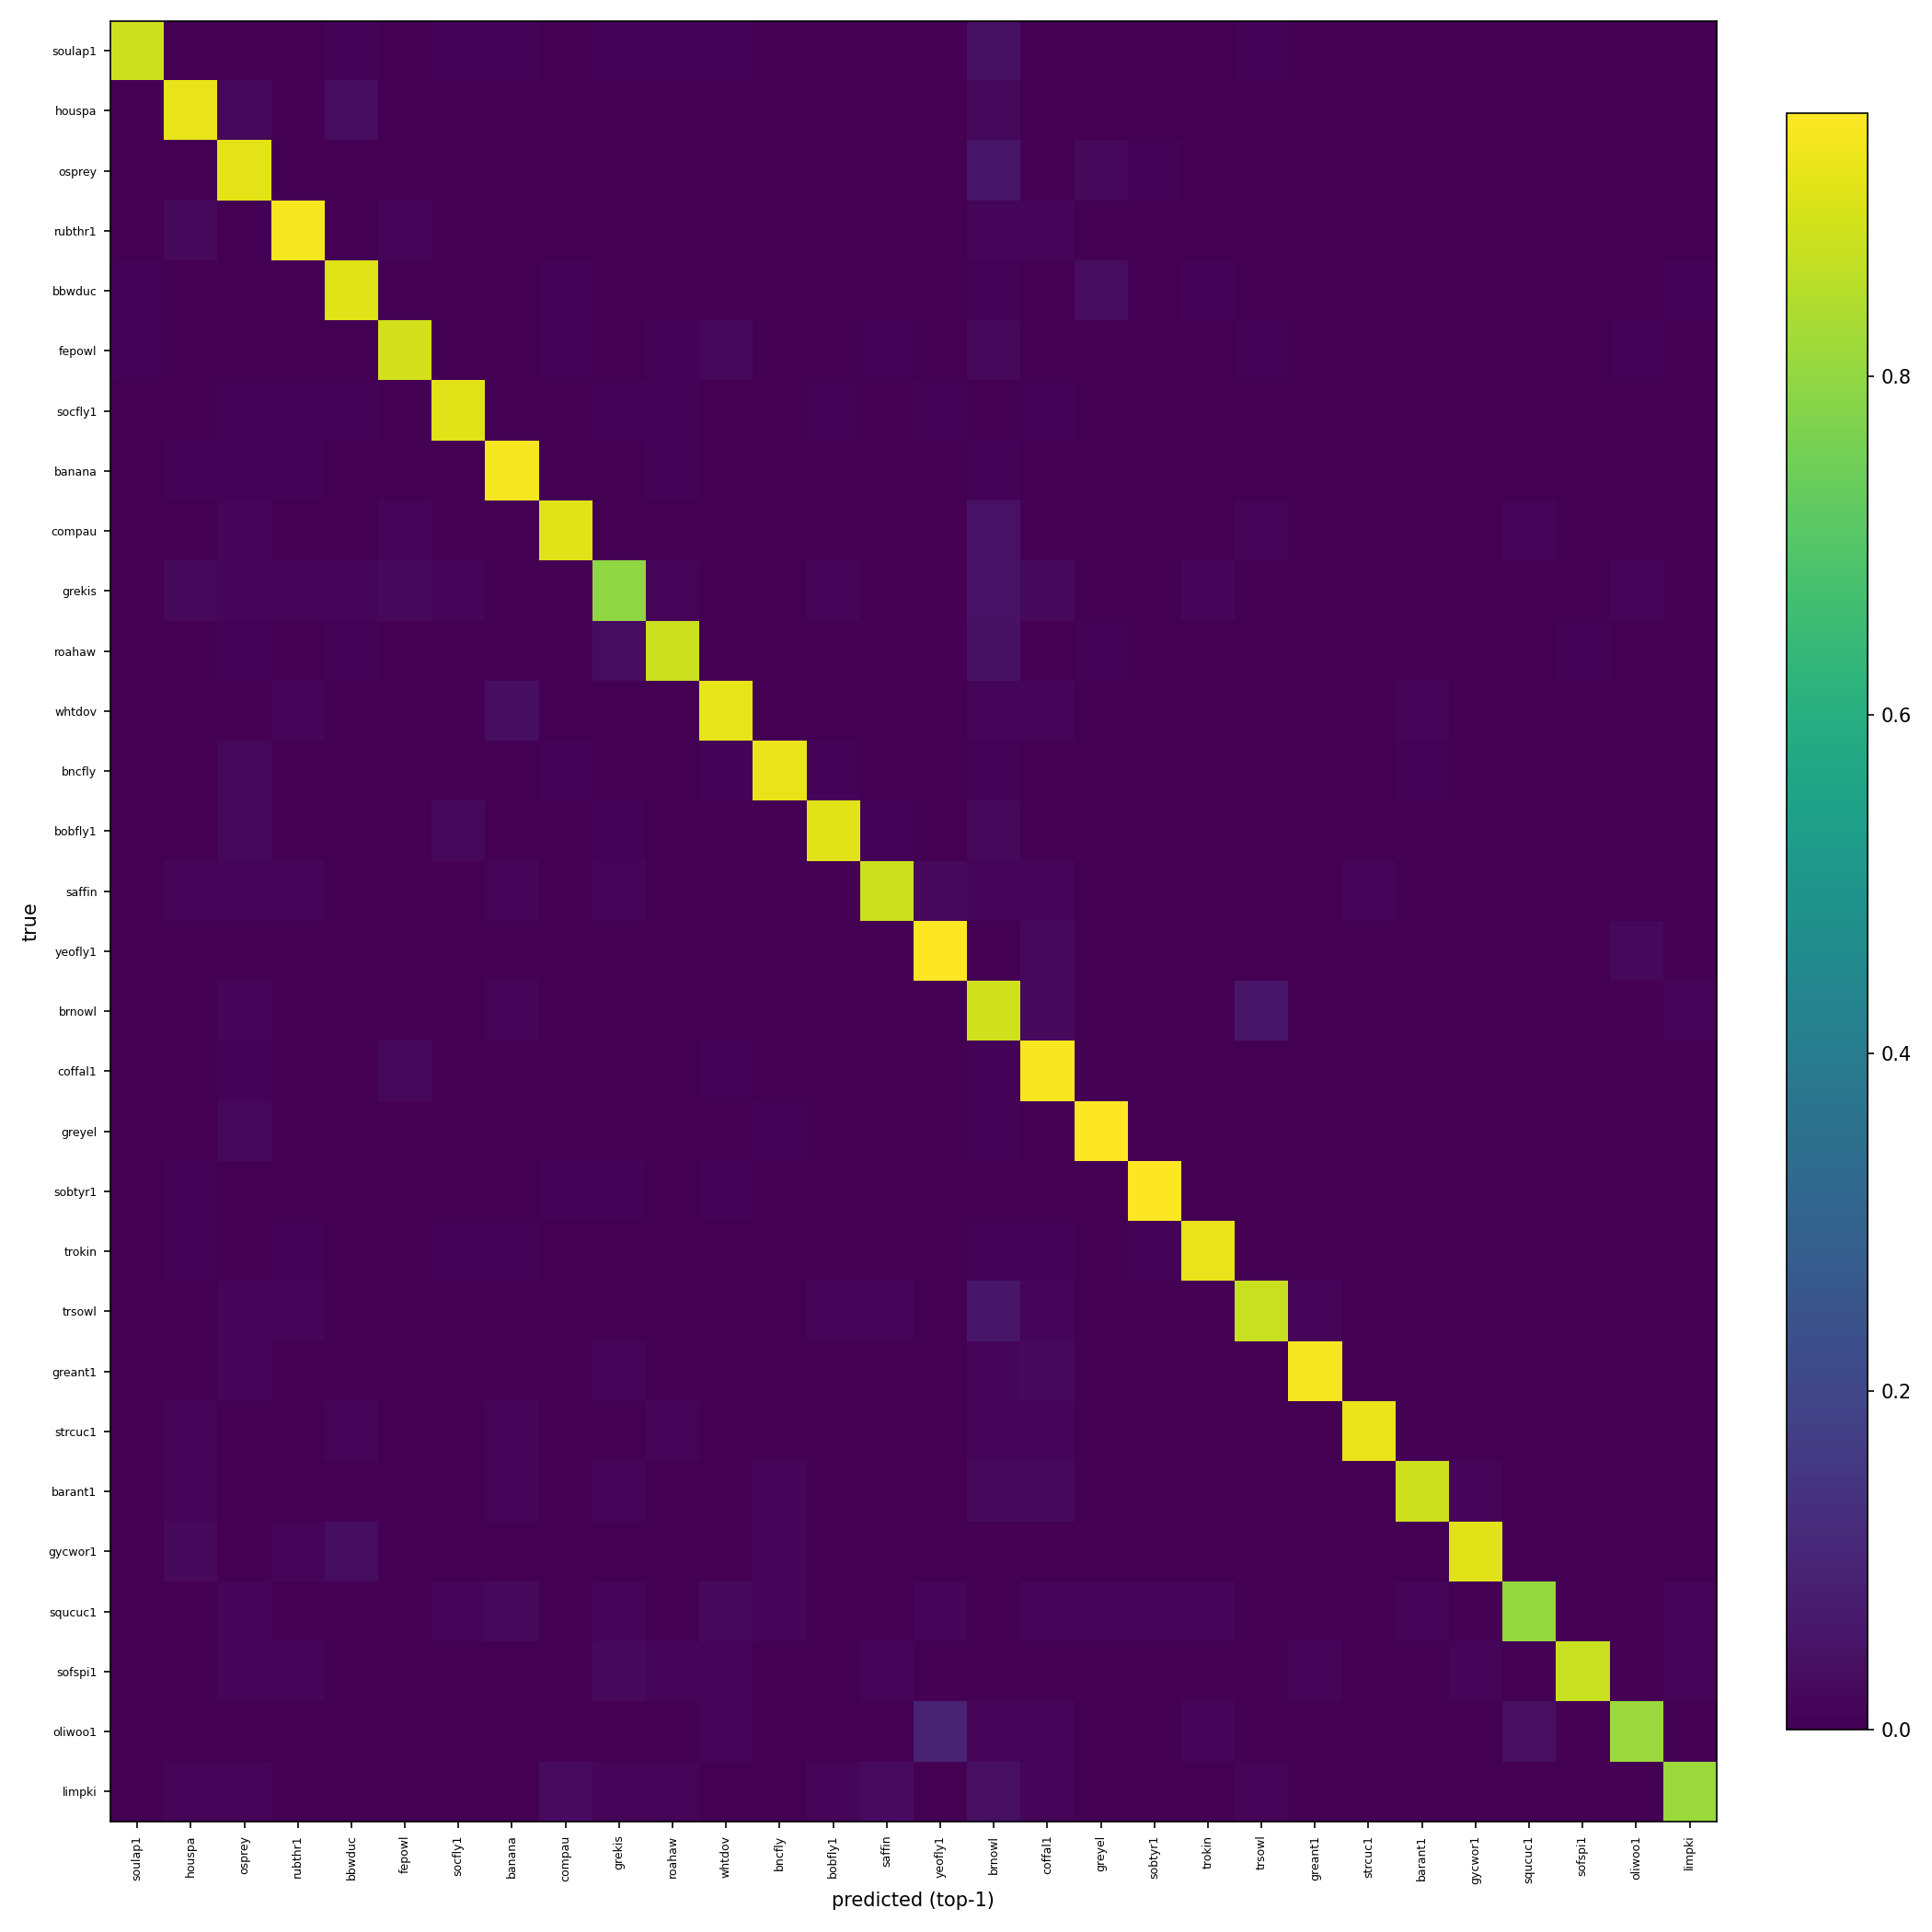
\includegraphics[width=\linewidth]{../results/strategy1_segments_torch/confusion.png}
    \caption{Matriz de confusões top-15 em E1 (Perch v2). Erros frequentes
    envolvem \texttt{brnowl} (coruja marrom) confundida com várias aves noturnas.}
    \label{fig:conf_e1}
  \end{minipage}
  \hfill
  \begin{minipage}{0.48\textwidth}
    \centering
    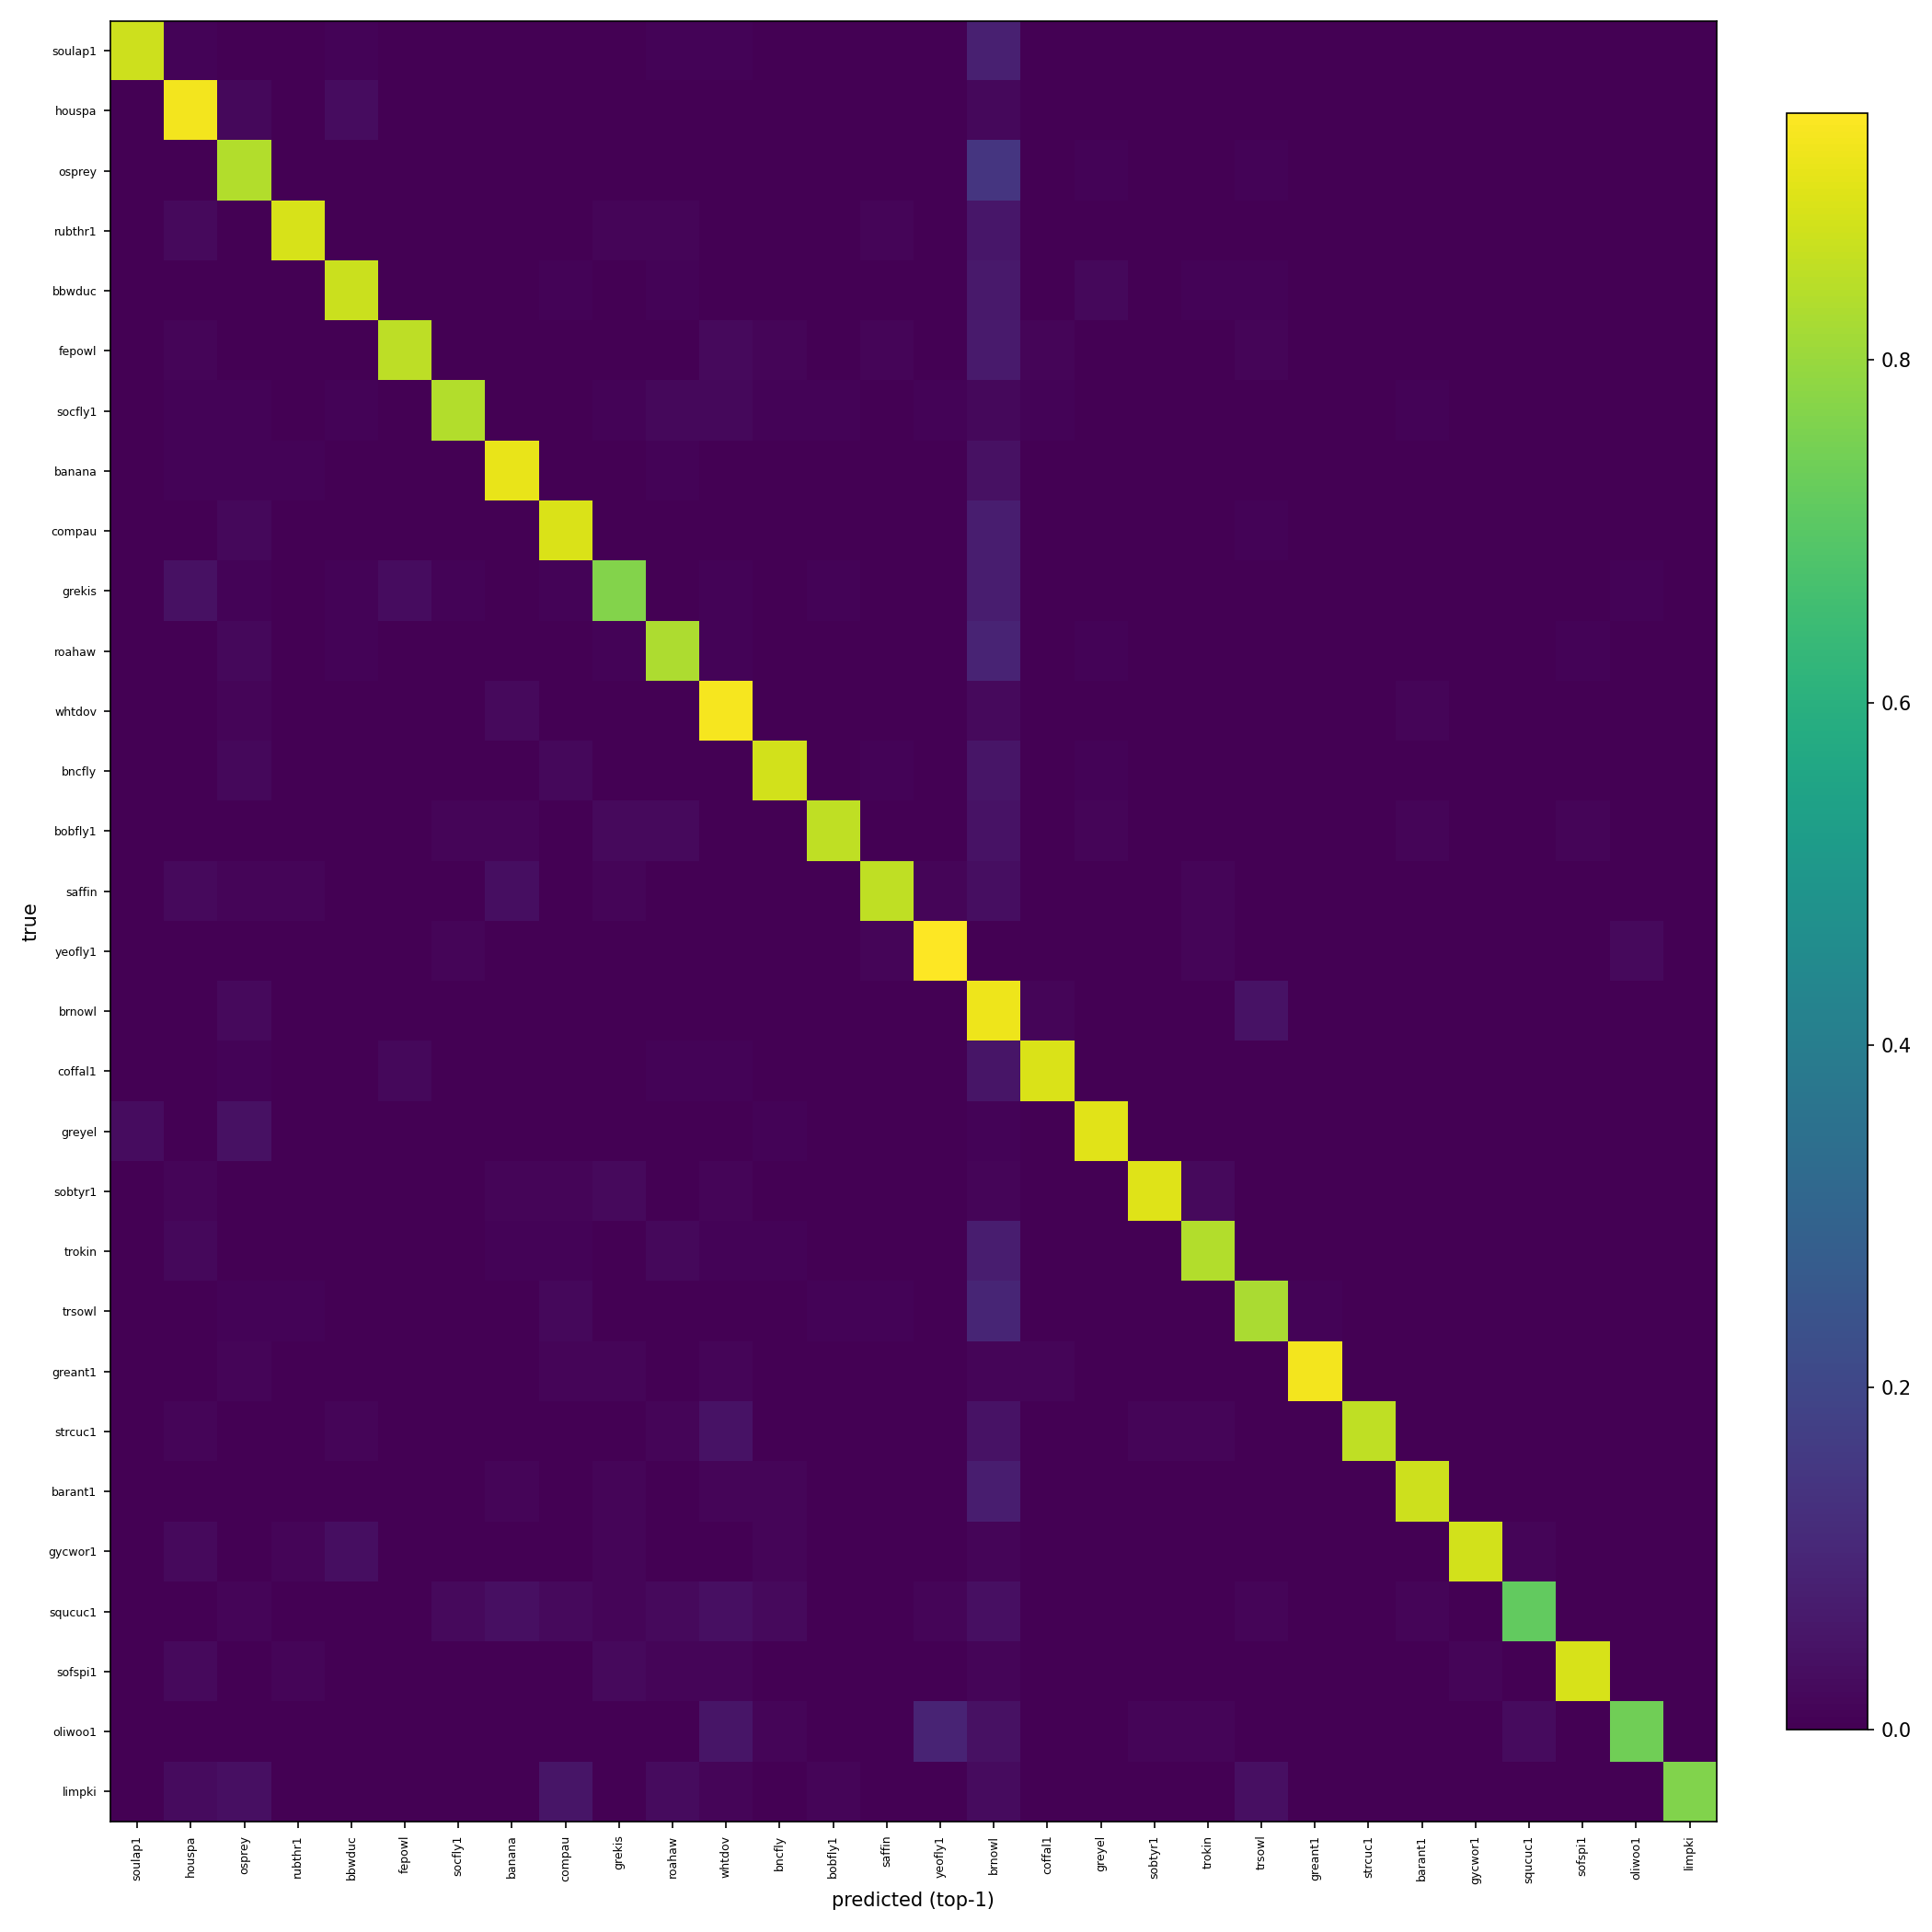
\includegraphics[width=\linewidth]{../results/strategy2_super_embedding_torch/confusion.png}
    \caption{Matriz de confusões top-15 em E2 (Perch v2). O super-embedding
    amplifica confusões com \texttt{brnowl}, aparecendo em 9 dos 15 pares.}
    \label{fig:conf_e2}
  \end{minipage}
\end{figure}

\subsection{Sweep de Rankers com Perch v2}

\begin{table}[htbp]
\centering
\caption{Resultados completos do sweep de rankers com Perch v2 (6.835 consultas).
Melhores valores em \textbf{negrito} por estratégia.}
\label{tab:sweep_perch_full}
\begin{tabular}{L{1.0cm}L{3.5cm}C{1.3cm}C{1.3cm}C{1.3cm}C{1.2cm}C{1.3cm}C{1.3cm}}
\toprule
\textbf{Est.} & \textbf{Ranker} & \textbf{MAP} & \textbf{MRR} & \textbf{nDCG} & \textbf{P@1} & \textbf{genus@5} & \textbf{Lat.\ ms} \\
\midrule
E1 & \texttt{attention} (T=0,05) & \textbf{0,8689} & \textbf{0,8689} & \textbf{0,8862} & \textbf{0,8269} & 0,9223 & 12,5 \\
E1 & \texttt{softmax} (T=0,1) & 0,8682 & 0,8682 & 0,8856 & 0,8252 & \textbf{0,9242} & 12,6 \\
E1 & \texttt{hybrid\_att\_sm\_tax} & 0,8691 & 0,8691 & 0,8862 & 0,8263 & 0,9247 & \textbf{1,0} \\
E1 & \texttt{taxonomy\_boost} & 0,8628 & 0,8628 & 0,8813 & 0,8180 & 0,9207 & 12,0 \\
E1 & \texttt{hybrid\_att\_rrf\_tax} & 0,8622 & 0,8622 & 0,8808 & 0,8202 & 0,9163 & 0,8 \\
E1 & \texttt{consensus\_ensemble} & 0,8629 & 0,8629 & 0,8817 & 0,8211 & 0,9172 & 1,2 \\
E1 & \texttt{rrf} ($k=60$) & 0,8179 & 0,8179 & 0,8406 & 0,7691 & 0,8844 & 11,9 \\
E1 & \texttt{borda} & 0,8170 & 0,8170 & 0,8403 & 0,7672 & 0,8832 & 11,9 \\
E1 & \texttt{rrf} ($k=30$) & 0,8256 & 0,8256 & 0,8480 & 0,7767 & 0,8913 & 11,8 \\
E1 & \texttt{topk\_mean} & 0,7632 & 0,7632 & 0,7890 & 0,7071 & 0,8375 & 12,0 \\
\midrule
E2 & \texttt{attention} (T=0,05) & \textbf{0,8494} & \textbf{0,8494} & \textbf{0,8694} & \textbf{0,8041} & \textbf{0,9131} & 5,1 \\
E2 & \texttt{hybrid\_att\_rrf\_tax} & 0,8476 & 0,8476 & 0,8677 & 0,8029 & 0,9069 & \textbf{0,3} \\
E2 & \texttt{softmax} & 0,8436 & 0,8436 & 0,8656 & 0,7925 & 0,9141 & 5,0 \\
E2 & \texttt{hybrid\_att\_sm\_tax} & 0,8467 & 0,8467 & 0,8665 & 0,7968 & 0,9156 & 0,3 \\
E2 & \texttt{taxonomy\_boost} & 0,8200 & 0,8200 & 0,8467 & 0,7561 & 0,9055 & 5,2 \\
E2 & \texttt{rrf} & 0,8227 & 0,8227 & 0,8457 & 0,7729 & 0,8907 & 5,0 \\
E2 & \texttt{topk\_mean} ($k=3$) & 0,8173 & 0,8173 & 0,8440 & 0,7681 & 0,8843 & 5,1 \\
\bottomrule
\end{tabular}
\end{table}

Os resultados na Tabela~\ref{tab:sweep_perch_full} revelam padrões consistentes:

\paragraph{Attention e Softmax dominam MAP/MRR.} Com Perch v2 em E1, o
\texttt{attention} (MAP\,=\,0,8689) e o \texttt{softmax} (MAP\,=\,0,8682)
apresentam ganho de $\approx$\,5 pontos sobre o \texttt{rrf} (0,8179). Isso
indica que a normalização por temperatura explora melhor a distribuição de scores
do Perch v2 do que a fusão por rank puro.

\paragraph{O híbrido att+sm+tax captura o melhor dos mundos.} O
\texttt{hybrid\_attention\_softmax\_taxonomy} alcança MAP\,=\,0,8691 em E1
--- marginalmente superior ao attention puro --- com latência de apenas 1,0~ms
(vs.\ 12,5~ms do attention). Isso ocorre porque os híbridos operam sobre as
listas de resultados já computadas, sem busca adicional no índice.

\paragraph{RRF performa abaixo do esperado.} O RRF, clássico em IR multimodal,
fica 5 pontos abaixo do attention (MAP 0,8179 vs.\ 0,8689). A hipótese é que o
Perch v2 produz scores de alta qualidade que carregam informação marginal além
da posição, e o RRF descarta essa informação ao usar apenas ranks.

\paragraph{Taxonomy Boost melhora genus@5.} O taxonomy\_boost alcança genus@5\,=\,0,9207
em E1, comparável ao softmax (0,9242). Sua força está em situações onde a espécie
exata não é identificada, mas o gênero é reconhecido.

\subsection{Sweep de Rankers com BirdNET v3.0}

\begin{table}[htbp]
\centering
\caption{Resultados selecionados do sweep de rankers com BirdNET v3.0
(6.835 consultas). Os resultados com BirdNET mostram padrão similar ao Perch v2,
com attention e softmax dominando.}
\label{tab:sweep_birdnet}
\begin{tabular}{L{1.0cm}L{3.5cm}C{1.3cm}C{1.3cm}C{1.3cm}C{1.2cm}C{1.5cm}}
\toprule
\textbf{Est.} & \textbf{Ranker} & \textbf{MAP} & \textbf{MRR} & \textbf{nDCG} & \textbf{P@1} & \textbf{Lat.\ ms} \\
\midrule
E1 & \texttt{attention} & \textbf{0,8944} & \textbf{0,8944} & \textbf{0,9105} & \textbf{0,8549} & 18,7 \\
E1 & \texttt{softmax} & 0,8910 & 0,8910 & 0,9078 & 0,8506 & 22,4 \\
E1 & \texttt{taxonomy\_boost} & 0,8894 & 0,8894 & 0,9064 & 0,8478 & 18,5 \\
E1 & \texttt{weighted\_topk} & 0,7743 & 0,7743 & 0,8029 & 0,7146 & 23,4 \\
E1 & \texttt{rrf} & 0,8312 & 0,8312 & 0,8555 & 0,7775 & 20,3 \\
E1 & \texttt{topk\_mean} & 0,7707 & 0,7707 & 0,8003 & 0,7083 & 16,7 \\
E1 & \texttt{hit} & 0,6743 & 0,6743 & 0,7270 & 0,5649 & 16,8 \\
E1 & \texttt{mean} & 0,2520 & 0,2520 & 0,2972 & 0,1671 & 17,3 \\
E1 & \texttt{median} & 0,2487 & 0,2487 & 0,2934 & 0,1649 & 17,8 \\
\midrule
E2 & \texttt{attention} & \textbf{0,8373} & \textbf{0,8373} & \textbf{0,8604} & \textbf{0,7881} & 6,2 \\
E2 & \texttt{softmax} & 0,8298 & 0,8298 & 0,8540 & 0,7786 & 6,0 \\
E2 & \texttt{rrf} & 0,8108 & 0,8108 & 0,8371 & 0,7557 & 5,9 \\
E2 & \texttt{taxonomy\_boost} & 0,8240 & 0,8240 & 0,8493 & 0,7700 & 6,2 \\
E2 & \texttt{topk\_mean} & 0,8076 & 0,8076 & 0,8332 & 0,7539 & 6,1 \\
E2 & \texttt{hit} & 0,2526 & 0,2526 & 0,3217 & 0,1504 & 6,9 \\
E2 & \texttt{mean} & 0,5163 & 0,5163 & 0,5973 & 0,3557 & 6,0 \\
E2 & \texttt{median} & 0,4560 & 0,4560 & 0,5382 & 0,3050 & 6,5 \\
\bottomrule
\end{tabular}
\end{table}

Com BirdNET, o \texttt{attention} em E1 alcança MAP\,=\,0,8944 --- o
\textbf{melhor resultado do projeto}, superando o Perch v2 em 2,55 pontos
percentuais. Isso sugere que o BirdNET produz embeddings com maior margem
entre espécies similares, beneficiando rankers que exploram os scores absolutos.

Um fenômeno notável é o colapso dos rankers \texttt{mean} e \texttt{median} com
BirdNET em E1 (MAP$\approx$\,0,25): o BirdNET produz scores mais extremos e
heterogêneos entre segmentos, e a média/mediana suprime os picos de sinal
relevantes. O \texttt{attention} e o \texttt{softmax}, que concentram o peso nos
picos, são imunes a esse problema.

\subsection{Comparação Global: Todos os Experimentos}

A Figura~\ref{fig:map_comparison} resume os MAPs de todos os experimentos.

\begin{figure}[htbp]
\centering
\begin{tikzpicture}
\begin{axis}[
    xbar,
    width=13cm, height=10cm,
    bar width=0.45cm,
    xlabel={MAP},
    xmin=0.20, xmax=0.95,
    ytick=data,
    yticklabels={
      {E1+BN+mean},
      {E1+BN+hit},
      {E1+PV+topk\_mean},
      {E1+BN+rrf},
      {E2+BN+rrf},
      {E1+PV+rrf},
      {E2+PV+tax\_boost},
      {E2+PV+attention},
      {E1+PV+tax\_boost},
      {E2+BN+attention},
      {E1+PV+softmax},
      {E1+PV+attention},
      {E1+BN+tax\_boost},
      {E1+BN+softmax},
      {E1+BN+attention}
    },
    nodes near coords,
    nodes near coords align={horizontal},
    every node near coord/.append style={font=\tiny},
    tick label style={font=\small},
    xlabel style={font=\small},
    grid=major, grid style={dashed, gray!30},
    legend style={at={(0.97,0.05)}, anchor=south east, font=\small},
  ]
  \addplot[fill=azul!40] coordinates {
    (0.252, 0) (0.674, 1) (0.763, 2) (0.831, 3)
    (0.811, 4) (0.818, 5) (0.820, 6)
    (0.849, 7) (0.863, 8)
    (0.837, 9) (0.868, 10) (0.869, 11)
    (0.889, 12) (0.891, 13) (0.894, 14)
  };
\end{axis}
\end{tikzpicture}
\caption{MAP dos principais experimentos. PV = Perch v2, BN = BirdNET v3.0.
O BirdNET com ranker Attention em E1 alcança o melhor MAP geral (0,894).}
\label{fig:map_comparison}
\end{figure}

\subsection{Análise de Latência}

\begin{figure}[htbp]
\centering
\begin{tikzpicture}
\begin{axis}[
    width=12cm, height=6cm,
    xlabel={Ranker},
    ylabel={Latência (ms)},
    xtick=data,
    xticklabels={rrf, attention, softmax, tax\_boost, hybrid\_att\_rrf, hybrid\_att\_sm},
    xticklabel style={rotate=30, anchor=east, font=\small},
    ybar,
    bar width=0.8cm,
    ymin=0, ymax=30,
    legend style={at={(0.97,0.97)}, anchor=north east},
    grid=major, grid style={dashed, gray!30},
    nodes near coords, nodes near coords align={vertical},
    every node near coord/.append style={font=\scriptsize},
  ]
  \addplot[fill=azul!50, draw=azul!80] coordinates {
    (1,11.9) (2,12.5) (3,12.6) (4,12.0) (5,0.8) (6,1.0)
  };
  \addplot[fill=verde!50, draw=verde!80] coordinates {
    (1,5.0) (2,5.1) (3,5.0) (4,5.2) (5,0.3) (6,0.3)
  };
  \legend{E1 (Segmentos), E2 (Super-Emb.)}
\end{axis}
\end{tikzpicture}
\caption{Latência média de busca por ranker. Híbridos atingem latência de
0,3--1,0~ms por operarem sobre listas pré-computadas, sem chamada adicional
ao índice. E2 é $\approx$\,2,4$\times$ mais rápido que E1 para rankers simples.}
\label{fig:latency}
\end{figure}

A Figura~\ref{fig:latency} mostra o perfil de latência. Rankers simples
(attention, softmax, rrf) têm latência dominada pelo custo da busca no índice
($\approx$\,12~ms em E1, 5~ms em E2). Rankers híbridos são drasticamente mais
rápidos ($<$\,1~ms) pois operam sobre os resultados já computados do índice
base, sem busca adicional.

\subsection{Análise de Confusões}

As confusões mais frequentes revelam padrões biologicamente interessantes:

\begin{itemize}
  \item \textbf{\texttt{brnowl} (coruja-café)} é a espécie mais confundida em E2,
  aparecendo em 9 dos 15 pares mais frequentes. Isso sugere que o super-embedding
  de \texttt{brnowl} fica próximo de muitas espécies noturnas no espaço de
  embedding, possivelmente devido à sobreposição de características espectrais
  de vocalizações noturnas.
  \item \textbf{\texttt{grfdov1} $\leftrightarrow$ \texttt{whtdov}} (pombas do gênero
  \textit{Columbina}/\textit{Zenaida}): confusão consistente em ambas as estratégias
  (8 ocorrências em E1, 13 em E2), indicando alta similaridade espectral entre
  essas espécies.
  \item \textbf{\texttt{oliwoo1} $\leftrightarrow$ \texttt{yeofly1}} (7 ocorrências):
  possivelmente vocalizações espectralmente similares de espécies de diferentes
  famílias.
\end{itemize}

O padrão dominante de confusões com corujas (\texttt{brnowl}, \texttt{trsowl},
\texttt{strowl1}) sugere que o espaço latente do Perch v2 agrupa espécies
noturnas próximas, o que pode ser explorado pelo \texttt{taxonomy\_boost} para
melhorar resultados biologicamente plausíveis.

\subsection{Resumo dos Trade-offs}

\begin{table}[htbp]
\centering
\caption{Síntese dos principais trade-offs de projeto no BirdSearch.}
\label{tab:tradeoffs_final}
\begin{tabular}{L{3.8cm}L{7.5cm}}
\toprule
\textbf{Decisão} & \textbf{Impacto Observado} \\
\midrule
Sobreposição 50\% & Essencial; remoção degrada MAP em 0,021--0,030 \\
\texttt{spectral\_gating} & Prejudicial neste contexto; reduz MAP em 0,049 (E1) \\
E1: fusão tardia (HNSW) & Melhor P@5 (+0,031); maior latência (22,6~ms); índice 13$\times$ maior \\
E2: fusão precoce (Flat) & Melhor MAP/P@1/nDCG; 3,5$\times$ mais rápido (6,3~ms) \\
Attention e Softmax & Melhor MAP/MRR nos dois backbones; $\tau=0{,}05$--$0{,}1$ \\
\texttt{taxonomy\_boost} & Melhor genus@5 (0,920--0,924); útil para proximidade biológica \\
Híbridos e Ensembles & MAP comparável a rankers simples; latência 10--40$\times$ menor \\
BirdNET \emph{vs.}\ Perch v2 & BirdNET superior em E1+attention (+0,026 MAP); scores mais extremos \\
\bottomrule
\end{tabular}
\end{table}

% ══════════════════════════════════════════════════════════════════════════════
\section{Conclusão}
\label{sec:conclusao}
% ══════════════════════════════════════════════════════════════════════════════

Este trabalho apresentou o \textbf{BirdSearch}, um sistema de recuperação de
informação acústica desenvolvido para o BirdCLEF 2026. O sistema implementa
um framework modular e config-driven que cobre integralmente o pipeline de RI:
pré-processamento, segmentação, embedding, representação, indexação, fusão e
reranking.

Os experimentos sobre o corpus completo (34.144 gravações, 571 espécies)
permitem extrair cinco conclusões principais:

\begin{enumerate}
  \item \textbf{A fusão precoce (E2) supera a fusão tardia (E1) no topo do
  ranking} (MAP 0,8227 \emph{vs.}\ 0,8191) e é 3,5$\times$ mais rápida (6,3~ms
  \emph{vs.}\ 22,6~ms). E1 mantém vantagem em P@5, preservando maior cobertura
  na lista expandida.

  \item \textbf{A sobreposição de 50\% é essencial}: vocalizações que cruzam
  fronteiras de janela só são corretamente representadas com overlap.

  \item \textbf{Rerankers baseados em score} (\texttt{attention} com $\tau=0{,}05$
  e \texttt{softmax} com $\tau=0{,}1$) superam consistentemente fusão por rank
  (RRF, Borda), com ganho de $\approx$\,5--8 pontos em MAP. O score absoluto do
  Perch v2 e do BirdNET carrega informação além da posição.

  \item \textbf{O BirdNET v3.0 alcança o melhor resultado do projeto}
  (MAP 0,8944, E1+attention), superando o Perch v2 por 2,55 pontos. Porém,
  rankers de aggregação simples colapsam com BirdNET (MAP $\approx$\,0,25),
  exigindo rankers que preservem picos.

  \item \textbf{Híbridos oferecem o melhor custo-benefício}: MAP comparável
  a rankers simples (0,8691 em E1) com latência de 0,3--1,0~ms, adequados para
  implantação em produção com restrições de tempo real.
\end{enumerate}

Como trabalhos futuros, identificam-se: (i) investigar filtros de ruído que
preservem as pistas espectrais discriminativas do Perch v2; (ii) explorar
\emph{fine-tuning} dos backbones sobre espécies amazônicas específicas do
BirdCLEF 2026; (iii) avaliar representações \texttt{cluster} e \texttt{prototype}
para capturar repertórios multi-modais; e (iv) implementar indexação dinâmica
(HNSW com inserções incrementais) para suporte a corpus crescentes de monitoramento
contínuo.

% ══════════════════════════════════════════════════════════════════════════════
\section*{Referências}
% ══════════════════════════════════════════════════════════════════════════════

\begingroup
\renewcommand{\section}[2]{}
\begin{thebibliography}{9}

\bibitem{merriënboer:25}
  van Merriënboer, B., Bhatt, R., Lostanlen, V., et~al.
  \textit{Perch: A Neural Embedding Framework for Bioacoustic Recognition}.
  arXiv:2312.09016, 2025.

\bibitem{kahl:21}
  Kahl, S., Wood, C.~M., Eibl, M., Klinck, H.
  \textit{BirdNET: A deep learning solution for avian diversity monitoring}.
  Ecological Informatics, 61, 101236, 2021.

\bibitem{cormack:09}
  Cormack, G.~V., Clarke, C.~L.~A., Buettcher, S.
  \textit{Reciprocal rank fusion outperforms condorcet and individual rank learning methods}.
  SIGIR 2009, pp.\ 758--759.

\bibitem{malkov:20}
  Malkov, Y.~A., Yashunin, D.~A.
  \textit{Efficient and robust approximate nearest neighbor search using Hierarchical Navigable Small World graphs}.
  IEEE TPAMI, 42(4), 824--836, 2020.

\bibitem{johnson:19}
  Johnson, J., Douze, M., Jégou, H.
  \textit{Billion-scale similarity search with GPUs}.
  IEEE Transactions on Big Data, 7(3), 535--547, 2021.

\bibitem{logothetis:96}
  Loizou, P.~C.
  \textit{Speech Enhancement: Theory and Practice}.
  CRC Press, 2007.

\bibitem{robertson:09}
  Robertson, S., Zaragoza, H.
  \textit{The Probabilistic Relevance Framework: BM25 and Beyond}.
  Found.\ Trends Inf.\ Retr., 3(4), 333--389, 2009.

\bibitem{jarvelin:02}
  Järvelin, K., Kekäläinen, J.
  \textit{Cumulated gain-based evaluation of IR techniques}.
  ACM TOIS, 20(4), 422--446, 2002.

\bibitem{baeza:99}
  Baeza-Yates, R., Ribeiro-Neto, B.
  \textit{Modern Information Retrieval}.
  ACM Press / Addison Wesley, 1999.

\end{thebibliography}
\endgroup

\end{document}
